\documentclass[11pt, oneside]{article} 
\usepackage{geometry}
\geometry{letterpaper} 
\usepackage{graphicx}
	
\usepackage{amssymb}
\usepackage{amsmath}
\usepackage{parskip}
\usepackage{color}
\usepackage{hyperref}

\graphicspath{{/Users/telliott_admin/Tex/png/}}
% \begin{center} 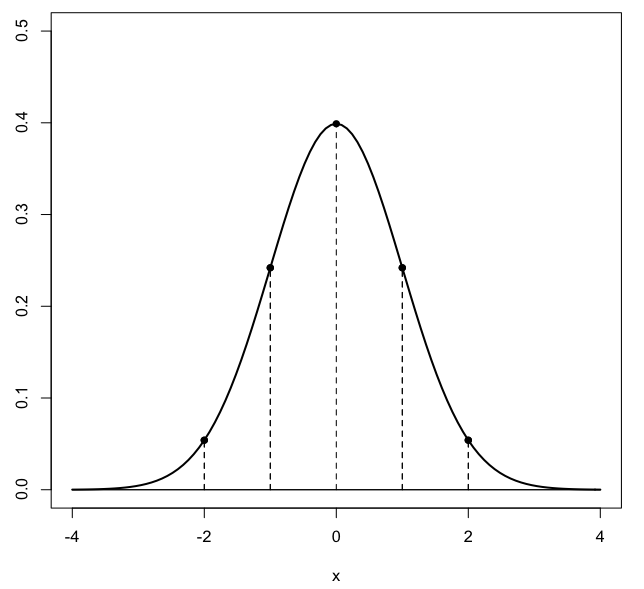
\includegraphics [scale=0.4] {gauss3.png} \end{center}

\title{Derivation of Green's Theorems}
\date{}

\begin{document}
\maketitle
\Large
The curl of $\mathbf{F}$ is defined to be
\[ \nabla \times \mathbf{F} = N_x - M_y \] 
for $\mathbf{F}=\ \langle M,N \rangle$.  

Curl measures how far the field is from being conservative.  Green's Theorem is
\[ \oint_C \mathbf{F} \cdot \mathbf{dr} = \iint_R \nabla \times \mathbf{F}  \ dA \]
\[ \oint_C M \ dx + N \ dy  = \iint_R (N_x - M_y) \ dA \]

where $\oint$ is an integral over a \emph{closed path}, traveling in the ccw direction.

The left-hand side "lives on the curve," whereas the right-hand side "lives over the whole region."

\section*{Derivation of Green's Theorem for Work}
\subsection*{1}

We will first show that
\[ \oint_C M \ dx = \iint_R -M_y \ dA \]
we are computing the special case where N = 0, there is only an x-component in the vector field.  But by symmetry 
\[ \oint_C N \ dy = \iint_R N_x \ dA \]
and the sum is equivalent to the theorem.

\subsection*{2}
Next, any complex curve (with some exceptions) can be decomposed into a set of regions, we do the integrals for each one, and the boundary curves between regions cancel.
\begin{center} 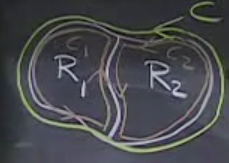
\includegraphics [scale=0.4] {regions.png} \end{center}

\subsection*{3}
So then finally, to prove:
\[ \oint_C M \ dx = \iint_R -M_y \ dA \]
We work on the line integral.  For a vertically simple region, we have a total of four curves going around.  The upper and lower curves are some functions $y = f_1(x)$ and $y = f_2(x)$.  We bound these with vertical lines.

\begin{center} 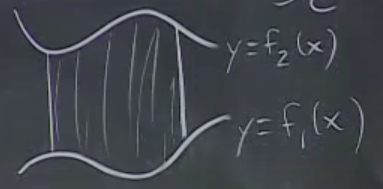
\includegraphics [scale=0.4] {Auroux22b.png} \end{center}

For the vertical segments $C_2$ and $C_4$ we have $dx=0$, the other two are
\[ \oint_C M \ dx = \oint_{C1} M \ dx + \oint_{C3} M \ dx \]
\[ =\int_a^b M(x, f_1(x)) \ dx - \int_a^b M(x,f_2(x)) \ dx \]

where $f_1$ is the lower curve and $f_2$ the upper one.  At each point along the curve, we have $y=f(x)$, so we can evaluate what $M(x,y)$ is at that point and then integrate with respect to $x$.  Notice that we have switched the bounds on the second integral, and added a minus sign.

Now look at the right-hand side in the theorem, the integral over the region 
\[ \iint_R -M_y \ dA = \iint_R -M_y \ dy \ dx \]
and
\[ M_y = \frac{\partial M}{\partial y} \]
so
\[ I = - \int_{x=a}^{x=b} \int_{y = f_1(x)}^{y = f_2(x)} \frac{\partial M}{\partial y} \ dy \ dx \]
but
\[ \frac{\partial M}{\partial y} \ dy = M \]

so the inner integral is just
\[ \int_{y = f_1(x)}^{y = f_2(x)} \frac{\partial M}{\partial y} \ dy = M(x, f_2(x)) - M(x, f_1(x)) \]

and  (remembering the minus sign) the outer integral is 
\[ - \int_a^b \ [ \ M(x, f_2(x)) - M(x, f_1(x)) \ ] \ dx \]

but that is the same as what we had above (taking account of the signs).

\section*{Derivation of Green's Theorem for Flux}
Green's Theorem for Flux has the same mathematical content as the work theorem, just substituting symbols to look at it in a different light.

The work theorem starts with
\[ \oint_C \mathbf{F} \cdot \mathbf{dr} = \int_C \mathbf{F} \cdot \hat{\mathbf{T}} \ ds \]
while the flux theorem starts with
\[ \int_C \mathbf{F} \cdot \hat{\mathbf{n}} \ ds \]
where
\[  d\mathbf{r} \cdot \hat{\mathbf{n}} = 0 \]

This formulation gave, for the work theorem
\[  \oint_C \mathbf{F} \cdot d\mathbf{r} = \int_C M \ dx + N \ dy = \iint_R (N_x - M_y) \ dA  \]

For the flux theorem the differentials have the same magnitude but they switch places and signs so that they will be orthogonal and thereby satisfy the condition $d\mathbf{r} \cdot \hat{\mathbf{n}} = 0$:
\[ \int_C \mathbf{F} \cdot \hat{\mathbf{n}}  \ ds = \langle M,N \rangle \cdot \langle dy,-dx \rangle = \int_C M \ dy - N \ dx \]

Rewrite with $dx$ first as usual.  
\[  \int_C - N \ dx +  M \ dy \]

Now apply Green's work theorem.
\[ \int_C -N \ dx + M \ dy  = \iint_R (M_x - (-N_y) \ dA = \iint_R (M_x + N_y) \ dA \]

As Strang says:  "playing with letters has proved a new theorem!...The components $M$ and $N$ can be chosen freely and named freely."

The left-hand side is
\[ \oint_C -N \ dx + M \ dy = \oint \mathbf{F} \cdot \hat{\mathbf{n}} \ ds \]
(recall that $\hat{\mathbf{n}} \ ds= \ \langle dy, -dx \rangle$).

while the right-hand side is
\[ \iint_R (M_x + N_y) \ dA = \iint_R \nabla \cdot \mathbf{F} \ dA \]

\subsection*{meaning of the divergence}
Green's theorem for flux says that

\[ \int_C \mathbf{F} \cdot \hat{\mathbf{n}} \ ds = \oint_C -N \ dx + M \ dy \]
\[ = \iint_R \nabla \cdot \mathbf{F} \ dA =  \iint_R M \ dx + N \ dy \]

The total flux or flow across the curve bounding the region R (heading to the outside) is equal to the \emph{divergence} of $\mathbf{F}$.  We obtain this result by a direct analysis, as follows.

We analyze the flow out of a small rectangle.  If $\mathbf{F}$ is continuously differentiable, then div $\mathbf{F}$ is is a continuous function, which is therefore approximately constant if the rectangle is small enough. The double integral is approximated by a product, since the integrand is approximately constant.

\begin{center} 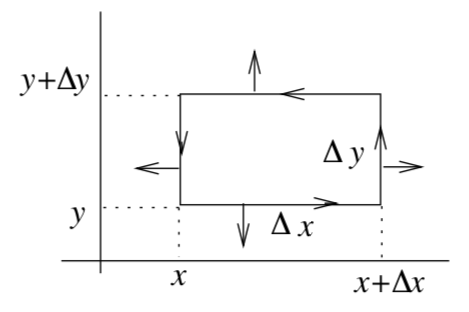
\includegraphics [scale=0.4] {divergence_derivation.png} \end{center}

The flux across the top is the part of $\mathbf{F}(x, y + \Delta y)$ in the $\mathbf{\hat{j}}$ direction times the length of the side:
\[  \mathbf{F}(x, y + \Delta y) \cdot \mathbf{\hat{j}} \ \Delta x = N(x,y + \Delta y) \ \Delta x \]
On the bottom we have a minus sign from the dot product and
\[  \mathbf{F}(x, y) \cdot \mathbf{\hat{j}} \ \Delta x = -N(x,y) \ \Delta x \]
Adding these two together
\[ N(x,y + \Delta y) \ \Delta x - N(x,y) \ \Delta x \approx (\frac{\partial N}{\partial y} \Delta y) \Delta x \]
An equivalent argument gives the flux across the sides as
\[ \approx (\frac{\partial M}{\partial x} \Delta x) \Delta y \]
So all four together yield
\[ (\frac{\partial N}{\partial y} \Delta y) \Delta x + (\frac{\partial M}{\partial x} \Delta x) \Delta y = (M_x + N_y) \Delta x \ \Delta y \]
which, in the limit as the rectangle becomes very small, is the divergence.  If we tile the region with tiny rectangles and sum them up, we obtain
\[ \iint_R (M_x + N_y) \ dx \ dy \]

\begin{quote}Continuing our search for a physical meaning for the divergence, if the total flux over the sides of the small rectangle is positive, this means there is a net flow out of the rectangle. According to conservation of matter, the only way this can happen is if there is a source adding fluid directly to the rectangle. If the flow is taking place in a shallow tank of uniform depth, such a source can be visualized as someone standing over the tank, pouring fluid directly into the rectangle. Similarly, a net flow into the rectangle implies there is a sink withdrawing fluid from the rectangle. It is best to think of such a sink as a “negative source”. The net rate (positive or negative) at which fluid is added directly to the rectangle from above may be called the “source rate” for the rectangle.\end{quote}

\begin{center} 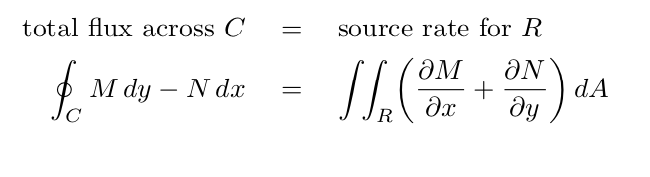
\includegraphics [scale=0.5] {Green_pic} \end{center}

\url{http://math.mit.edu/~jorloff/suppnotes/suppnotes02/v4.pdf}

\end{document}  